\subsection{Effect of Strategy Conditioning on Exploration}
\label{sec:strategy-exploration-ablation}

We compare a Qwen3-8B coder conditioned on a frozen strategist with the same
coder generating directly from the problem and parent context. We compare
construction-level exploration over a shared training horizon at a matched
coder-attempt budget, with parent selection evolving independently in each run.

Figure~\ref{fig:strategy-exploration-ablation} shows diverging exploration
patterns as training progresses. Without the strategist, the coder
increasingly reproduces selected parents, while distinct non-parent
constructions become rare. Strategy conditioning maintains a lower
parent-copy rate and continues to yield distinct alternatives later in
training. The main benefit observed here is therefore sustained
construction-level exploration: the frozen strategist provides guidance
that helps the adapting coder move beyond reproducing existing parents.

\begin{figure*}[t]
    \centering
    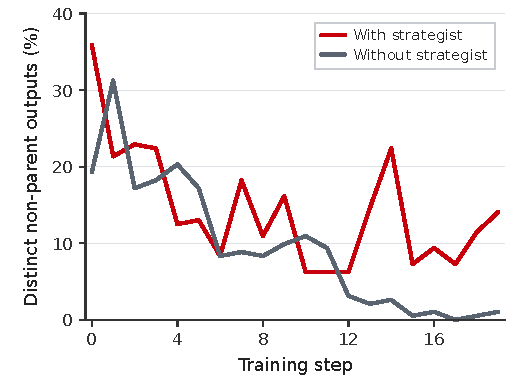
\includegraphics[width=0.49\textwidth]{output/pdf/strategy_exploration_comparison_diversity.pdf}
    \hfill
    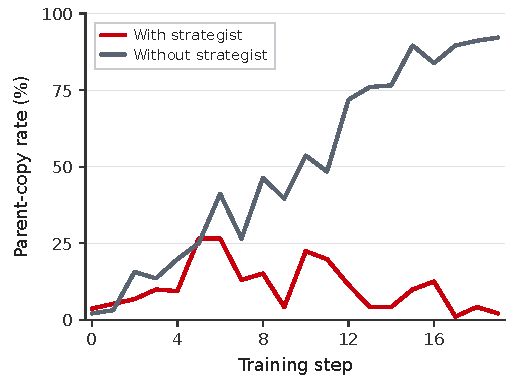
\includegraphics[width=0.49\textwidth]{output/pdf/strategy_exploration_comparison_parent_reproduction.pdf}
    \caption{\textbf{Strategy conditioning and construction-level exploration.}
    Left: distinct valid constructions that differ from every selected
    parent, counted once per step. Right: valid outputs equivalent to any
    selected parent, counting repeated copies. Both are normalized by all
    coder attempts, including failures. Matching uses normalized
    piecewise-constant constructions with tolerance $10^{-8}$, treating
    reflection and complementation as equivalent.}
    \label{fig:strategy-exploration-ablation}
\end{figure*}
